%++++++++++++++++++++++++++++++++++++++++
% Don't modify this section unless you know what you're doing!
\documentclass[letterpaper,12pt]{article}
\usepackage[utf8]{inputenc}
\usepackage{float}
\usepackage{tabularx} % extra features for tabular environment
\usepackage{amsmath}  % improve math presentation
\usepackage{graphicx} % takes care of graphic including machinery
\usepackage[margin=1in,letterpaper]{geometry} % decreases margins
\usepackage{cite} % takes care of citations
\usepackage[final]{hyperref} % adds hyper links inside the generated pdf file
\usepackage[table,xcdraw]{xcolor}
\hypersetup{
	colorlinks=true,       % false: boxed links; true: colored links
	linkcolor=blue,        % color of internal links
	citecolor=blue,        % color of links to bibliography
	filecolor=magenta,     % color of file links
	urlcolor=blue         
}
%++++++++++++++++++++++++++++++++++++++++


\begin{document}

\title{Práctica 4 - Ruteo Externo}
\author{Matthew Aguerreberry, Natasha Tomattis}
\date{\today}
\maketitle

% \begin{abstract} 
% \end{abstract}


\section{Practica de Ruteo Externo - BGP}
	% \begin{figure}[ht] 
			
	% 	\centering 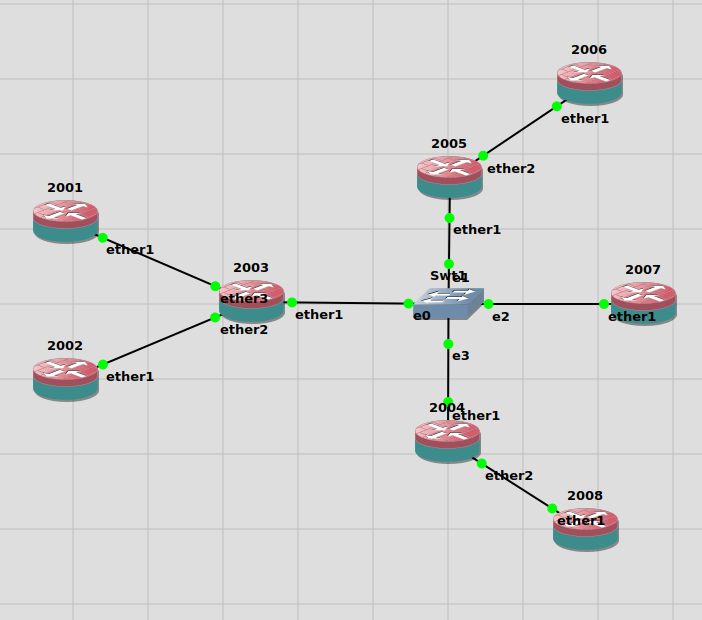
\includegraphics[width=0.8\columnwidth]{figure/topo_figura1.png}
	% 	\caption{
	% 			\label{fig:samplesetup} % spaces are big no-no 
	% 			Implementación Ejercicio 1.
	% 	}
	% \end{figure}
	\begin{enumerate}
		\item \textbf{Conectar los routers segun el diagrama de la figura 1.}
		\item \textbf{Configurar las interfaces de acuerdo al diagrama. Definir las redes loopbacks para simular redes internas (en el AS 5692 las loopbacks estan en el router 5692C).}
		\item \textbf{Configurar eBGP e iBGP segun corresponda. Comprobar que se establecen las sesiones correctamente entre los routers vecinos. No habilitar BGP en el router 5692C} \\
		\item \textbf{Que protocolo de capa de transporte utiliza BGP? Que puerto usa? Capturar trafico para responder estas preguntas}\\
		\begin{figure}[H] 
			
			\centering 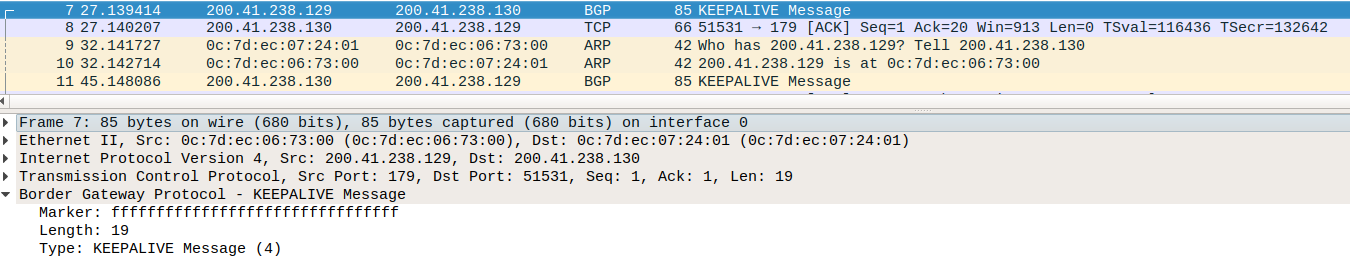
\includegraphics[width=0.5\columnwidth]{figure/bgp-transport.png}
			\caption{
					\label{fig:samplesetup} % spaces are big no-no 
					Captura de mensajes BGP en la interfaz ether2 en el router 5962A.
			}
		\end{figure}
		\item \textbf{Que mensajes intercambian dos routers vecinos para establecer una sesion BGP?}\\
		\begin{figure}[H] 
			
			\centering 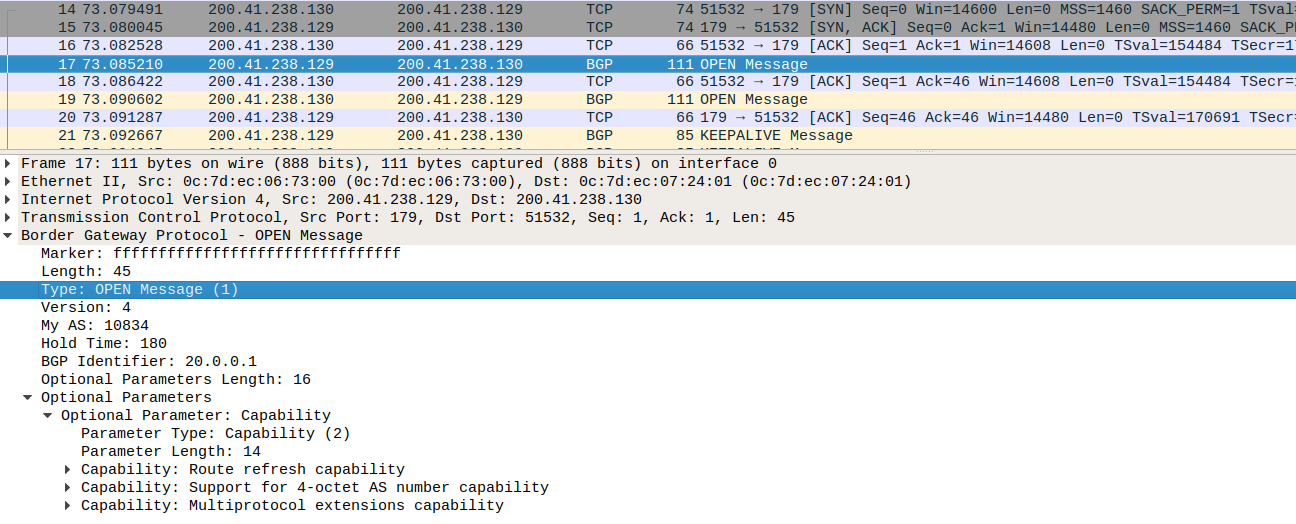
\includegraphics[width=0.5\columnwidth]{figure/bgp-open.png}
			\caption{
					\label{fig:samplesetup} % spaces are big no-no 
					Captura de mensajes BGP en la interfaz ether2 en el router 5962A.
			}
		\end{figure}
		\item \textbf{Cuales son los estados en los que se pueden encontrar una sesion BGP?}\\
	
	
	\end{enumerate}

	\subsection{Enlaces consultados}
		\begin{itemize}
			\item{HCNA Networking Study Guide}  \\
			\textit{Springer. Huawei Technologies Co., Ltd.},Ch 8.2 RIP.
			\item \href{https://www.juniper.net/documentation/en_US/junos/topics/concept/ospf-stub-áreas-overview.html}
			{Understanding OSPF Stub Areas, Totally Stubby Areas, and Not-So-Stubby Areas}
			\item \href{https://www.juniper.net/documentation/en_US/junos/topics/concept/ospf-routing-external-metrics-overview.html} 
			{Understanding OSPF External Metrics}
			\item \href{https://wiki.mikrotik.com/wiki/Manual:Routing/OSPF}
			{Manual:Routing/OSPF}

		\end{itemize}
\end{document}